The ball and beam system shown in the figure below is a popular
platform for control experiments.
\begin{exerfig}
  \action*{RMM}{Replace figure with xfig version}
  \centering\footnotesize
  \psfrag{x}[][]{$q_2$}
  \psfrag{f}[][]{$q_1$}
  \psfrag{P}[][]{$P$}
  \psfrag{a}[][]{$a$}
  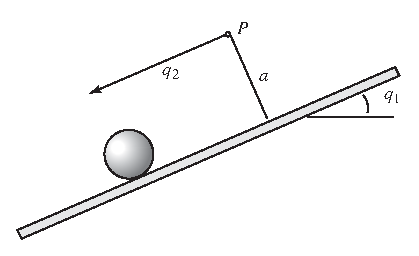
\includegraphics{\exerdir/ballbeam.eps} 
\begin{fignotes}
{\bf PUP}: Pivot point $P$ should be closer to the center of the beam
and there should be a visible pivot (either a point on the beam of a
triangular pivot that the beam rotates on top of).
\end{fignotes}
\end{exerfig}
The system consists of a beam that rotates around the pivot $P$, its
angle is controlled by a motor. The ball moves in a grove on the beam.
The goal is to control the position of the ball on the beam. The
dynamics are similar to the dynamics of the vector thrust vehicle
discussed in Example~\ref{examp:modeling:pvtol-modeling}. Introduce
the state variables beam angle $q_1$ and ball position $q_2$ as shown
in the figure and let the torque from the motor be $T_m$. Show that
the system can be modeled by the following equations
\begin{displaymath}
  \bmat{J_{1e}+m_2q_2^2&m_{12}\\m_{12}&m_{2e}}\ddot q+\bmat{2m_2\dot q_1\dot q_2\\m_2\dot q_1^2q_2}+g\bmat{ml_e\sin{q_1}-m_2q_2\cos{q_1}\\m_2\sin{q_1}}=\bmat{T_m\\0}
\end{displaymath}
where $J_e$, $m_{12}$, $m_e$ and $ml_e$ are constant parameters.
\begin{comment}
\begin{displaymath}\aligned
J_{1e}&=J_1+m_1l_1^2+J_2+m_2l_2^2\\
m_{12}&=J_2/r+m_2l_2\\
m_{2e}&=J_2/r^2+m_2\\
ml_e&=m_1l_1+m_2l_2\\
l_2&=a+r
\endaligned\end{displaymath}  
\end{comment}
The mass matrix is nonlinear because it depends on the position of the
ball, the nonlinear damping term represents Coriolis\index{Coriolis
forces} and centripetal 
forces and the spring term represents the effects of gravity. It is also
implicitly assumed that the ball is in contact with the beam at all
times.

\begin{solution}
  The equations of motion can be conveniently derived using Lagrange's
  equations (see~\cite{Can03}). To do this we start by accounting for
  the potential and kinetic energy of the system.

The potential energy of the ball and the beam is
\begin{displaymath}
  V=-m_1gl_1\cos{q_1}-m_2gl_2\cos{q_1}-m_2gq_2\sin{q_1},
\end{displaymath}
where $m_1$ and $m_2$ are the masses of beam and ball respectively, $l_1$ is the distance from the pivot to the center of mass of
the beam, $l_2=a-r$, where $a$ is the distance from the pivot to
the center of the rolling track and $r$ the rolling radius of the beam.

The kinetic energy of the beam is
\begin{displaymath}
  T_1=\frac{1}{2}J_1\dot q_1^2+\frac{1}{2}m_1l_1^2\dot q_1^2.
\end{displaymath}
To compute the kinetic energy of the ball we first compute the
velocity of its center of mass. We have in a fixed coordinate system
with the origin at the pivot point
\begin{displaymath}
  x_1=-q_2\cos{q_1}+l_2\sin{q_1},\qquad x_2=-q_2\sin{q_1}-l_2\cos{q_1},
\end{displaymath}
hence
\begin{displaymath}\aligned
  \dot x_1&=-\dot q_2\cos{q_1}+q_2\dot q_1\sin{q_1}+l_2\dot q_1\cos{q_1}\\ 
  \dot x_2&=-\dot q_2\sin{q_1}- q_2\dot q_1\cos{q_1}+l_2\dot
  q_1\sin{q_1}\\
  v^2&=\dot x_1^2+\dot x_2^2=l_2^2\dot
  q_1^2-2l_2\dot q_1\dot q_2+\dot q_2^2+\dot q_1^2q_2^2=\bigl(l_2\dot q_1+q_2\bigr)^2+(q_2\dot q_1)^2.
\endaligned\end{displaymath}
The kinetic energy of the ball is
\begin{displaymath}
  T_2=\frac{1}{2}J_2\Bigl(\dot q_1+\frac{\dot
    q_2}{r}\Bigr)^2+\frac{1}{2}m_2\bigl(l_2^2\dot
  q_1^2+2l_2\dot q_1\dot q_2+\dot q_2^2+\dot q_1^2q_2^2\bigr).
\end{displaymath}
The Lagrangian is $L=T_1+T_2-V$ and its partial derivatives are:
\begin{displaymath}\aligned
\frac{\partial L}{\partial q_1}&=-m_1gl_1\sin{q_1}-m_2gl_2\sin{q_1}+m_2gq_2\cos{q_1}\\
\frac{\partial L}{\partial q_2}&=m_2g\sin{q_1}+m_2q_2\dot q_1^2\\
\frac{\partial L}{\partial\dot q_1}&=
(J_1+m_1l_1^2+J_2+m_2l_2^2+m_2q_2^2)\dot
q_1+\bigl(J_2/r+m_2l_2\bigr)\dot q_2\\
\frac{\partial L}{\partial\dot
  q_2}&=\bigl(J_2/r+m_2l_2\bigr)\dot q_1+(J_2/r^2+m_2)\dot q_2.
\endaligned\end{displaymath}
The equations of motion are now obtained using Lagrange's equations
\begin{displaymath}
  \frac{d}{dt}\frac{\partial L}{\partial\dot q_i}-\frac{\partial
    L}{\partial q_i}=T_i,
\end{displaymath}
and we get
\begin{displaymath}\aligned
&(J_1+m_1l_1^2+J_2+m_2l_2^2+m_2q_2^2)\ddot
q_1+\bigl(J_2/r+m_2l_2\bigr)\ddot q_2+2m_wq_2\dot q_1\dot
q_2\\&m_1gl_1\sin{q_1}+m_2gl_2\sin{q_1}-m_2gq_2\cos{q_1}=T_m\\
&\bigl(J_2/r+m_2l_2\bigr)\ddot q_1+(J_2/r^2+m_2)\ddot q_2-m_2g\sin{q_1}-m_2q_2\dot q_1^2
\endaligned\end{displaymath}
Introducing
\begin{displaymath}\aligned
J_e&=J_1+m_1l_1^2+J_2+m_2l_2^2 &m_{12}=J_2/r+m_2l_2\\
m_e&=J_2/r^2+m_2 &ml_e=m_1l_1+m_2l_2
\endaligned\end{displaymath}
gives the state equations. 

An experimental system at Lund University has the parameters
$m_1=$\unit{1.5}{\kilo\gram}, $m_2=$\unit{0.53}{\kilo\gram} and the
moments of of beam and ball (with respect to centers of mass)
$J_1=$\unit{0.12}{\kilogram\meter^2} and $J_2=$\unit{1.3\cdot
  $10^{-4}$}{\kilogram\meter^2} . The shortest distance from the pivot
point to the track is $a=$\unit{0.03}{\meter}, the distance from the
pivot to the center of mass of the beam is $l_1=$\unit{0.035}{\meter}
and the rolling radius of the ball is $r=$\unit{0.05}{\meter}. The
current constant is $k_i=$\unit{0.6}{\newton\meter/\ampere}, the
maximum current is \unit{4.5}{\ampere}. In the real system there is
also damping that can be modeled linearly.

\end{solution}
\begin{comment}
\begin{displaymath}
  M(q)\ddot q+C(q,\dot q)+K(q)=\bmat{T\\0}
\end{displaymath}
where
\begin{displaymath}\aligned
m_{11}&=J_{beam}+m_{beam}l^2+J_{ball}+m_{ball}((a_r)^2+r^2\theta^2)\\m_{12}&=J_{ball}+m_{ball}rl_2,\quad\quad
m_{22}=J_{ball}+m_{ball}r^2
\endaligned\end{displaymath}
and
\begin{displaymath}
 C=m_{ball}r^2\bmat{\dot\varphi\dot\theta\\m_{ball}\theta\dot\varphi^2},\qquad K=\bmat{(m_{beam}l+m_{ball}l_2)g\sin{\varphi}+m_{ball}gr\theta\cos{\varphi}\\m_{ball}gr\sin{\varphi}}  
\end{displaymath}
\begin{displaymath}
  M=\bmat{J_{beam}+&J_{ball}^{cm}+m_{ball}rl_2\\J_{ball}^{cm}+m_{ball}rl_2&J_{ball}^{cm}+mr^2},\quad C=m_{ball}r^2\bmat{\dot\varphi\dot\theta\\m_{ball}\theta\dot\varphi^2}
\end{displaymath}
\begin{displaymath}
  M=\bmat{a_{11}+m_2q_2^2&a_{12}\\a_{12}&a_{22}},\qquad\bmat{c_1\dot q_1\dot q_2\\c_2\dot q_1^2q_2},\qquad\bmat{k_{11}\sin{q_1}+k_{12}\cos{q_1}\\k_2\sin{q_1}}
\end{displaymath}  
\end{comment}

